\documentclass[tudarticle,type=msc,colorback,accentcolor=tud9c]{tudthesis}

  \usepackage[utf8]{inputenc}
  \usepackage[thmmarks]{ntheorem}
  \usepackage{xspace,cleveref,xcolor}
  \usepackage{amsmath}
  \usepackage{graphicx,url}
  \usepackage[font=small]{caption}
 \usepackage{subcaption}
 \usepackage[parfill]{parskip}

% new commands
  \newcommand{\QQ}{\mathbb Q}
  \newcommand{\RR}{\mathbb R}
  \newcommand{\CC}{\mathbb C}
  \newcommand{\NN}{\mathbb N}
  \newcommand{\ZZ}{\mathbb Z}
  \newcommand{\DD}{\mathbb D}
  \newcommand{\A}{\mathcal A}
  \newcommand{\B}{\mathcal B}
  \newcommand{\C}{\mathcal C}
  \newcommand{\D}{\mathcal D}
  \newcommand{\R}{\mathcal R}
  \newcommand{\M}{\mathcal M}
  \newcommand{\laplace}{\operatorname\Delta}
  \bibliographystyle{plain}

  \newcommand{\p}{\ensuremath{\mathcal P}\xspace}
  \newcommand{\np}{\ensuremath{\mathcal{NP}}\xspace}
  \newcommand{\fp}{\ensuremath{\mathcal{FP}}\xspace}
  \newcommand{\abs}[1]{\left|#1\right|}
  \newcommand{\sharpp}{\ensuremath{\# \mathcal{P}}\xspace}
  \newcommand{\code}{\texttt}
  \newcommand{\cc}{\code{C++}\xspace}
  \newcommand{\ccx}{\code{C++11}\xspace}
  \newcommand{\irram}{\code{iRRAM}\xspace}
  \newcommand{\MPFR}{\code{MPFR}\xspace}
  \newcommand{\baana}{\code{BA\_ANA}\xspace}
  \newcommand{\anarect}{\code{ANA\_RECT}\xspace}
  \newcommand{\powerseries}{\code{POWERSERIES}\xspace}
  \newcommand{\poly}{\code{POLY}\xspace}
  \newcommand{\func}{\code{FUNC}\xspace}
  \newcommand{\real}{\code{REAL}\xspace}
  \newcommand{\temp}{\textcolor{red}}
  \newcommand{\seq}{\mathbf}
  \DeclareMathOperator{\lb}{lb}
  \DeclareMathOperator{\bigo}{O}
  \newcommand{\sprec}{prec\xspace}
  \newcommand{\demph}{\textbf}
  \newcommand{\sdzero}{\texttt{0}}
% ntheorem environments
  \theoremseparator{:}
  \theorembodyfont{\itshape}
  \newtheorem{definition}{Definition}[section] 
  \theorembodyfont{\upshape}
  \newtheorem{theorem}{Theorem}[section] 
  \newtheorem{corollary}{Corollary}[section] 
  \newtheorem{example}{Example}[section]
  \newenvironment{proof}{\paragraph{Proof:}}{\hfill$\square$}
\begin{document}
  \thesistitle{Case Studies in Exact Real Arithmetic - Implementations and empirical Evaluation}{Fallstudien in exakter reeller Arithmetik: Implementation und empirische Evaluation}
  \author{Holger Thies}
  \referee{Prof. Dr. Martin Ziegler}{tba}[tba]
  \department{Mathematics}
  \group{Mathematical Logic}
  \dateofexam{\today}{\today}
  \makethesistitle
  \affidavit{H. Thies}
\dedication{Danksagung...}
\begin{abstract}
    Abstract...
\end{abstract}  
\tableofcontents
  \chapter{Introduction}

  \chapter{Theoretical Background}
  \section{Floating Point Arithmetic and Real Numbers}
  %!TEX root = ../../thesis.tex
\section{Real Computability Theory}\label{sec:real computability}
\subsection{Classical Computability Theory}
 Since in real computability theory many aspects of classical computability theory are extended, 
 a very brief overview is given in the following section.

 To define computability the Turing-Machine model is used.
 The Turing-Machine was invented by Alan Turing in 1936 \cite{Turing} and can
 be seen as simplified mathematical model for a computer.

 The machine constists of an infinite tape that is divided into cells. 
 Each cell contains exactly one symbol from a predefined finite alphabet
 $\Sigma$.
 It further consists of a head that is always positioned on top of one cell 
 and can in one step read and write the content of the cell and then move one
 cell left or right on the tape.

 The machine is always in one of finitely many states and has a finite
 instruction table containing instructions of the form when in state $q$ and
 reading symbol $s$, write $s'$ and move head to the left (or to the right).

 A formal definition can for example be found in \cite{Hopmann}.
 
 \begin{definition}
 	A possibly partial function $f:\subseteq \Sigma^* \to \Sigma^*$ is called \textbf{computable} if there exists 
 	a Turing-Machine, so that for all $x \in dom(f)$ the machine terminates after finitely many steps with $f(x)$ on its 
 	tape and for $x \not \in dom(f)$ the machine does not terminate.
 \end{definition}

 Even tough the Turing-Machine model is quite simple, it can be used to
 simulate every computer algorithm.
 The widely believed \textbf{Church-Turing thesis} even states, that anything
 that is computable in an informal sense, can be computed with a
 Turing=machine.

 The following definitions for sets also play a very important role in
 computability theory:
 \begin{definition}
 	A set $A \subseteq \Sigma^*$ is called \textbf{decidable}, if its characteristic function is computable. 
 \end{definition}
 \begin{definition}
 	A set $A \subseteq \Sigma^*$ is called \textbf{recursively enumerable} (r.e.) or \textbf{computably enumerable} (c.e.) if 
 	it is empty or if $A$ is the domain of a computable function.   
 \end{definition}
\subsection{Computability of real numbers}
The previous section showed how to define computability over finite alphabets $\Sigma^* \to \Sigma^*$. 
That is enough to define computability for finite structures. The following section defines how to extend 
the classical notion to uncountable objects such as real or complex numbers, functions or infinite sequences.
There are several non equivalent ways, to define computability on such objects. 
In contrast to the classical case, where the definition given in the previous section is widely accepted, there is no 
generally accepted model for real complexity theory.

The model used in this thesis is the so called \textbf{Type 2 Theory of Effectivity} (TTE). 
Because... 

This section gives an overview of the framework used to define computability on real numbers and is therefore 
a little more general then needed in the rest of the thesis, that focuses more on implementations of subsets of this framework.
However,...

The general definition is by Type-2 Turing Machines...
From now on the term Turing-Machine is used both for classical and type 2 machines, when it is clear by context which model is meant.
\begin{definition}\label{def:computability_ttt}
A function $F:\subseteq \Sigma^\omega \to \Sigma^\omega$ is called computable if there is a Turing-Machine  
that for all infinite strings $\sigma in dom(F)$ writes the infinite string $F(\sigma)$ on its output tape. 
For $\sigma \not \in dom(f)$ the machine writes only finitely many symbols on the output tape.  
\end{definition}
To talk about computability over some set, the notion of encoding this set to $\sigma^\omega$ has to be formalized.
\begin{definition}\label{def:representation}
	A \textbf{representation} of a set $X$ is a partial surjective mapping $\alpha: \sigma^\omega \to X$. \\
	$\bar \sigma \in \alpha^{-1}(\sigma)$ is called an \textbf{$\alpha$-name} of $\sigma$. \\
	$x \in X$ is \textbf{$\alpha$-computable} if it has a decidable $\alpha$-name.
\end{definition}

Of course, the definition of representations is open wide and can lead to many different more or less useful definitions of computability.
Some possible representations for real numbers are as follows
\begin{enumerate}
\item A $\rho_{10}$-name of $x$ is the usual decimal expansion of $x$.
\item A $\rho$-name of $x \in \RR$ is a sequence $a_n \in \ZZ$ s.t. $| x - a_n | \leq 2^{-n}$
\item  A $\rho_C$-name of $x \in \RR$ consists of two sequences rational $(q_n)_{n \in \NN}$ and $(\varepsilon_n)_{n \in \NN}$, so that 
$| x_n - q_n | < \varepsilon_n$ and $\lim_{n \to \infty} \varepsilon_n = 0$  
\item $\rho_<$-name, $\rho_>$-name
\item $\rho_n$-name 
\end{enumerate}
\begin{theorem}
The following are equivalent
\item $x \in \RR$ is computable in the sense of Definiton 
\item $x \in \RR$ is $\rho_{10}$ computable
\item $x \in \RR$ is $\rho$-computable
\end{theorem}
\begin{example}
Specker-Sequence
\begin{definition}\label{def:representation_composition}
Composition of representations
\end{definition}
\end{example}
This thesis does not deal with the problem of computing single real numbers, but rather with computing real functions and real functionals.
For a function $f:\subseteq \RR \to \RR$ to be computable means, that is it possible to compute $f(x)$ arbitrarily good. 
Also a machine can not read $x$ with infinite precision, but it can ask to get $x$ as exact as it needs it to compute the output.
\begin{definition}\label{def:computability_oracle_tm}
\end{definition}
This concept can be generalized by the following definiton  
\begin{definition}\label{def:computability_function_representation}
	A function $f: \subseteq X \to Y$ is called \textbf{$(\alpha, \beta)$}-computable, 
	if there exists a computable function $F:\subseteq \Sigma^\omega \to \Sigma^\omega$ such that 
	$\beta(F(\sigma)) \in f(\alpha(\sigma))$ for all $\sigma \in dom(f \circ \alpha) $.  
\end{definition}
The Diagram in ... shows computability.
Examples...
\begin{theorem}
Multiplication is not $(\rho_{10}, \rho_{10})$-computable.
\end{theorem}
From now on the term computable will be used to describe computability w.r.t. the Cauchy representation.
Then all of the following functions are computable
\begin{enumerate}
\item Arithmetical operations $+,-,x,/ : \subseteq \RR^2 \to \RR$
\item The absolute value function
\item The minimum and maximum functions
\item constant functions with computable constant
\item Projections $\RR^k \to \RR$ 
\item polynomials with computable coefficients
\item $exp, sin, cos$
\item The square-root function and the logarithm function
\end{enumerate}
\begin{theorem}
	Computable functions are continuous...
\end{theorem}

\begin{theorem}
Computability is preserved under function composition, i.e.
For sets $X,Y,Z$ with representations $\delta_X, \delta_Y, \delta_Z$, 
$f:\subseteq X \to Y$ $(\delta_X, \delta_Y)$-computable and $g:\subseteq Y \to Z$ $(\delta_Y, \delta_Z)$-computable,
$g \circ f$ is $(\delta_X, \delta_Z)$-computable.
\end{theorem}
\begin{definition}
A multi-valued function $f: \subseteq X \rightrightarrows Y$ is just an other name for a relation $f \subseteq X \times Y$.
A multi-valued function is $(\rho_X, \rho_Y)$ computable, if there is a a comnputable (single valued) function 
$F: \subseteq \Sigma^\omega \to \Sigma^\omega$ such that for all $\sigma \in dom(f \circ \rho_X)$, $\rho_Y(F(\sigma)) \in f(\rho_X(\sigma))$. 
\end{definition}
\subsection{Computability of real operators and functionals}
A real operator maps functions $\RR \to \RR$ to functions $\RR \to \RR$and a functional maps functions $\RR \to \RR$ to real numbers $\RR$.
For that, a representation for the space to work on is needed.
Continuous functions on a compact subset $X \subseteq R^d$ can be uniformly approximated by polynomials arbitrarily close.
A possible representation for real valued functions is thus given by the following definition 
\begin{definition}
A $[\rho^d \to \rho]$-name of a function $f \in C([0,1]^d, \\R)$ is given by a sequence $P_n \in \\D[x1, \dots, x_d]$ of polnomials (i.e. degree and list of coefficients), such that $\vert f - P_n \vert_\infty < 2^{-n}$   
\begin{theorem}[name?]
The integration operator 
$$I: C[0,1] \ to C[0,1], f \to (x \to \int_0^x f(t) dt$$   
is computable.
\end{theorem}
\begin{theorem}[Myhill 1971]
There is a computable function $f: [0,1] \to \R$ with continuous but uncomputable derivative. 
\end{theorem}
\begin{theorem}
The operator 
$$ D: C^1[0,1] \to C[0,1], f \to f'$$
is computable.
\end{theorem}
\end{definition}
\subsection{Uniformity and Non-Uniformity}
When talking about computability one has to distinguish between two types of computability, \textbf{uniform} and \textbf{non-uniform}.
FOr non-uniform computability it suffices, that for every input, there is an algorithm that computes the output. 
The algorithm may however depend on the input in a non-computable way.
In contrast, a problem is uniformly computable only if there is one algorithm, that computes the output for every valid input. 
Intermediate Value Theorem
\subsection{Other models for comoutable reals}
Markov Computability \\ 
Sequential Computabilty \\
Computable invariance \\
BSS-model \\

  %!TEX root = ../../thesis.tex
\section{Real Complexity Theory}\label{section:real_complexity}
	\subsection{Classical Complexity Theory}
    In contrast to computability theory, complexity theory deals with the
    question how many resources (in form of e.g. time or space) are needed to
    compute a computable function.

    Again, the Turing-Machine model is used to describe the computations
		\begin{definition}
			For a given Turing Machine $M$ and $w \in \Sigma^*$, $time_M(w)$ is the number of head movements 
			the Turing Machine on input $w$ exectues before it terminates. \\
			For $n \in \NN$ define $time_M(n) = \max \{ time_M(w) \,|\, w \in \Sigma^* and M terminates on input w \}$.\\
			Analogously, one can define space constraints.
		\end{definition}
    In most cases it is not important to compute the exact running time, but
    one rather wants to approximate how the algorithm will behave when the
    input is getting large.
    The standard way to compare the asymptotic running time of algorithms is
    the use of $O$-notation.
		\begin{definition}
			For functions $f, g: \NN \to \NN$ one writes $f \in O(g(n))$ if there are constants $M \in \RR$, $n_0 \in \NN$, such that
			$ f(n) \leq M \cdot g(n)$ for all $n > n_0$. 
		\end{definition}
			Thus, for a given algorithm a way to measure its complexity is giving an
      upper bound on its worst case running time for inputs of length $n$ in
      terms of the $O$-notation. 

			However, complexity theory mainly is not about the complexity of specific
      algorithms, but rather deals with the complexity of problems. 
      That is, trying to classify the complexity of \textbf{any} algorithm to
      decide a subset of $\Sigma^*$.
      
      The following gives a classifications of problems depending on the
      running time for algorithms solving those problems.
		\begin{definition}
			For a function $t: \NN \to \NN$ let 
      $$ \text{DTIME}(t) = \{ A \subseteq \Sigma^* \,|\, \text{There is a
      Turingmachine } M \text{ deciding } A \text{ with time}_M(n) \in O(t(n)) \} $$

      NTIME$(t)$ describes the same for the case of $M$ being a
      non-deterministic Turing-machine.
		\end{definition}
		The above definitions suffice to define the most important complexity classes
		\begin{definition}
			The complexity classes $P, NP, PSPACE$ and $EXPTIME$ are defined as follows:
			\begin{eqnarray*}
				P & := & \bigcup_{k \in N} DTIME(n^k) \\
				NP & := & \bigcup_{k \in N} NTIME(n^k) \\
				PSPACE & := & \bigcup_{n \in N} DSPACE(n^k) \\
				EXPTIME & := & \bigcup_{k \in N} DTIME(2^{n^k}) \\
			\end{eqnarray*}
		\end{definition}
		It holds $P \subseteq NP \subseteq PSPACE \subseteq EXPTIME$. 
		It is $P \neq EXPTIME$ and for all other inclusions it is not known if equality holds, but most 
		complexity theorists consider it as extremely unlikely.

    Another way to characterize the important class $NP$ is the following
    \begin{theorem}
      $A \subseteq \Sigma^*$ is in $NP$ if and only if there are polynomials
      $p$ and $q$ and a deterministic Turing-Machine $M$ such that for all $x
      \in \Sigma^*$ with length n, there is an $y \in \Sigma*$ with length
      bounded by $q(n)$ such that $x \in A \text{ iff } M(<x,y>) = 1$ and 
      $x \not \in A \text{ iff } M(<x,y>) = 0$. 
      Further $M$'s running time is bounded by $p(n)$ for all such inputs
      $<x,y>$.  
    \end{theorem}
		Wheter $P = NP$ is one of the Millenium problems and one of the biggest unsolved problems in Computer Science.

		One can also consider function problems instead of decision problems
    leading to a dual hierarchy of complexity classes.
		\begin{definition}
      A functional problem $F: \Sigma^* \rightrightarrows \Sigma^*$, is solved
      by a Turing-Machine in if it writes on every $x \in \Sigma^*$ an output
      $z \in F(x)$ or decides that no such output exists.  \\ Time- and
      Space-Complexity can be defined accordingly. \\ The classes $FP$ and
      $FPSPACE$ are defined as the class of polynomial time resp. space
      computable functions. \\ The class $\#P$ is defined as the the class of
      functions that give the number of solutions to a problem in $NP$.
    \end{definition}
		It holds $FP \subseteq \#P \subseteq FPSPACE$ and if $FP = \#P$ would hold, it would follow that $P = NP$.
     
		Problems that are known to be in $P$ are often considered as the feasible functions, 
		for which it is possible to find an efficient algorithm. 

    Since most of the complexity classes are not known to be distinct, they do
    not suffice to classify problems by their difficulty.
    To compare the difficulty of problems, reductions are used.
		\begin{definition}
			$A \subset \Sigma^*$ is \textbf{polynomial time reducible} to $B \subseteq \Sigma^*$ ($A \leq_P B)$, 
			if there is a polynomial time computable function $f; \Sigma^* \to \Sigma^*$, such that
			$$ w \in A \Leftrightarrow f(w) \in B.$$
		\end{definition}
		Many other types of reductions exist, e.g. to compare complexity classes
    lower then $P$, but they are not needed in this thesis and therefore
    omitted.

		The hardest problems in a complexity class are called complete for this class
		\begin{definition}
			A set $A \subseteq \Sigma^*$ is called \textbf{$\C$-hard} (w.r.t. $\leq_P$) for a complexity class $\C$, if for all $B \in \C$ $B \leq_P A$. \\
			$A$ is called \textbf{$\C$-complete} (w.r.t. $\leq_P$), if $A$ is $\C-hard$ and $A \in \C$.  
		\end{definition}
		If one would show for a single $\C$-complete problem that it is in $P$, it would follow that all problems in $\C$ are in $P$.
		Consequently a way to show that there is most likely no efficient algorithm to a problem, is to show that the problem is $NP$-hard.
    For many problems it could be shown that they are $NP$-complete. 
    Some of the most important ones can for example be found in
    \cite{bookwithnpcompleteproblems}
	\subsection{Complexity Theory on real numbers}
		In classical complexity theory the time complexity is usually measured in terms of the input size.
		However, when considering continuous peoblems, the input is an infinite string and thus can not 
		be used to measure the running time of an algorithm.

		In numerical computations an important parameter is the desired output precision.
		Thus, it seems reasonable to analyze the running time as a function depending on the desired output precision.
    
		This leads to the following definition for the complexity of a single real
    number
		\begin{definition}\label{def:complexity_real_number}
			A real number $x \in \RR$ is computable in time $t$ if there is a Turing Machine $M$ that with input $n \in \NN$ in binary, 
			outputs the binary expansion of a dyadic rational number $d$ with $| x - d | \leq 2^{-n}$.  
		\end{definition}
		Again this notion can be generalized by using representations and type-2
    Turing machines, i.e. by considering the time that is needed to write the first $n$ symbols
		of the name of the output.
      
    One has to be careful, however, since representations that are
    computationally equivalent, do not necessary lead to the same complexity
    bounds.  For example, one can construct arbitrarily long Cauchy names for
    any rational number.
    Thus, it is not even possible to define the complexity of a real number
    with respect to its Cauchy name.

		A more useful representation for complexity is the signed-digit
    representation.
		\begin{definition}
			The \textbf{signed digit representation} $\rho_sd$ is defined as follows: 

			A $\rho_d$-name of a real number $x$ is a sequence 
			$$a_n a_{n-1} \dots a_0 . a_{-1} a_{-2} \dots \text{ with } a_i \in \{-1,0,1\}, n \geq -1, a_n \neq 0, a_n + a_{n-1} \neq 0$$
      and
			$$  x = \sum_{i=n}^{-\infty} a_i \cdot 2^i $$  
		\end{definition}
		As with the binary expansion, the number digits after the binary point correspond to the precision.

		\temp{The advantage to the binary expansion is that, the signed digit
    representation is symmetric, ,,,}
		It can be shown that the signed digit representation is computably equivalent to the Cauchy representation.

		When extending the complexity notion to functions, apart from the output
    precision, an additional parameter might be interesting: the precision of the input
		needed to compute the output up to the demanded precision.

    This leads to the following definition
		\begin{definition}
      A function $f: \subseteq \RR \to \RR$ is computed on a compact set $K
      \subseteq dom(f)$ in time $t$ with lookahead $l$ if for all
      $\rho_{sd}$-names of elements $ x \in K$ by a Turing Machine $M$ if $M$
      computes a $\rho_{sd}$-name of $f(x)$ and after t steps and with reading
      at most $l$ symbols of the input string outputs the $n$-th symbol of the
      output.   
    \end{definition} 
    The above comolexity notion really only makes sense on a compact set, since
    otherwise the machine could already spend arbitrarily much time on just
    reading the input left from the binary point.
    
    An alternative approach to define complexity of functions is using Oracle
    Turing Machines which have polynomial time bounded running time. 

    With the above notion computable real numbers and functions can be
    classified into complexity classes like in the discrete case.
    An important class for practical purposes is the class of polynomial time
    computable numbers and functions, since they usually can be computed
    efficiently with a computer.
   
    An important property of polynomial time computable reals is given in the
    following theorem.
		\begin{theorem}[Ko and Friedmann]
			The set of polynomial time computable real numbers forms a real algebraically closed field.
		\end{theorem}
		\begin{example}
     The following real valued functions are polynomial time computable on a compact set
     $K$
     \begin{enumerate}
       \item Addition, Subtraction and Multiplication as functions $K \times K
         \to \RR$.
        \item The function $x \mapsto \frac(1){x}$ if $0 \not in K$. 
         \item The functions $\exp, \sin, \cos$ as functions $K \to \RR$.
     \end{enumerate}
		\end{example}
	\subsection{Complexity of Operators}
		Since most interesting function spaces such as $C[0,1]$ are not locally compact,
		there is no straight forward way to generalize the above definitions to get
    a uniform notion of complexity for operators.

		In fact, the following holds
		\begin{theorem}
      Even restricted to continuous functions $f: [0,1] \to [0,1]$, the
      evaluation operator $x \to f(x)$ is not computable within time uniformly
      bounded in terms of the output error only.  
    \end{theorem}

	  A different approach to study the complexity of operators and functionals
    is followed by Ko and Friedman \cite{KoBook}.
    Instead of trying to define a complexity notion for a functional $F$, they
    study the time complexity of the real valued function $F(f)$ where $f$ is a
    polynomial time computable function.


		This  method leads to many connections between discrete complexity classes
    and numerical problems,

    One example of such a connection is given in the following theorem.
		\begin{theorem}[Friedman \cite{Fri}]
			The following are equivalent
			\begin{enumerate}
				\item $FP = \#P$
				\item For every polynomial time computable function $f: [0,1] \to \R$, the function
					$g: [0,1] \to \R$, defined by $g(x) = \int_0^x f(t) dt$ is polynomial time computable.
			\end{enumerate} 
		\end{theorem}
		Thus, one can say that integration of polynomial time computable functions is at
    least as hard as solving a problem in $\#P$.
    In that sense, Integration can be called $\#P$-hard.

    \temp{Maybe add something on second order representations}
 	\subsection{Parameterized Complexity}
  \temp{Write something or remove this section.}

  \chapter{iRRAM}
  \section{Real Number representation}
  \section{Overview of Classes}
  \section{Multivalued Functions}
  \section{Similiar Frameworks}

  \chapter{Case Studies}
  %!TEX root = ../../thesis.tex
\section{Dynamic Systems and the Shadowing Lemma}
\subsection{Introduction}
  \begin{definition}
    A \textbf{discrete dynamical system} is a triple $(\NN,X,\Phi)$ with $X$ a non empty set (the state space) and an operation $\Phi : \NN \times X \to X$, so that
    $\Phi(0,x) = x$ and $\Phi(n,\Phi(m,x)) = \Phi(n+m, x)$. 
    Thus, a discrete dynamical system is the model of a system, that evolves over discrete time steps.
  \end{definition}
  The simplest case of a discrete dynamical system, is when the state space is 1-dimensional (say $X \subseteq \RR$) and 
  the transition function only depends on the previous value, i.e. $\Phi(1,x) = f(x)$ for some $f : \RR \to \RR$. 
  Then the dynamical system can be written by the recurrence relation $x_{n+1} = f(x_n)$ with initial condition $x_0 \in \RR$.
  A chaotic system is a dynamical system, that is highly sensitive to initial conditions.
  A consequence of that is that even relatively small numerical errors in the computation grow exponentially fast.
  A prototypical example of a chaotic system is the logistic map:
  \begin{definition}\label{def:logmap}
    The \textbf{logistic map} is given by the recurrence relation 
    $ x_{n+1} = ax_n(1-x_n) \text{ with } a, x_0 \in \RR$.
  \end{definition} 
  \begin{table}
    \begin{tabular}{ | c | c | }
    \hline
    $a$ & behaviour \\ \hline
    $[0,1]$ & Stabilizes at $0$ \\ \hline
    $(1,3]$ & Stabilizes at $\frac{a-1}{r}$ \\ \hline 
    $(3, \approx 3.544]$ & oscillates between $2$, $4$, $8$, $\dots$ values. \\ \hline 
    $(\approx 3.544, 4]$ & \begin{tabular}{l}almost all inital points no oscillation with finite period \footnote{This is true for most points in this interval. There are however isolated ranges of $a$ for which the oscillation period is finite.}  \\ Small changes in the initial point yield large differences over the iterations. \end{tabular} \\ \hline
    $(4, \infty)$ & The values eventually leave the interval [0,1] and diverge for almost all initial points \\ 
    \hline
    \end{tabular}
    \caption{behaviour of iterating the logistic map for different values of the parameter $a$}\label{table:logmapbehaviour}
  \end{table}
  The logistic map behaves differently for different values of the parameter $a$ as can be seen in Table \ref{table:logmapbehaviour}. 
  The for this thesis interesting case is for $a \in (3.544, 4)$ where the iteration of the map leads to chaotic behaviour.

  Since the \irram framework can be used to compute iterations of the logistic map exactly, it is very well suited to invesitgate this chaotic behaviour \footnote{what could also be shown in a contest in 2000 \cite{competition:2001}}. 

  Figure \ref{fig:logmaperror1} shows how sensitive the map is to small errors that occur because of finite precision computations. 
  When using 10 significant digits for the computation, it can be seen that after around 50 iterations the finite precision version diverges from the \irram version and then behaves completely differently. 

  \irram can also be used to approximate the complexity in terms of needed computation precision. Since \irram automatically increases the internal precision until it suffices to output the result with the demanded number of digits, the internal precision at the end of the computation gives a measure of this complexity. As can be seen in Figure \ref{fig:logmapprec}, the needed internal precision grows extremely quickly with the number of iterations.
  To compute 10 significant digits of the $20000$-th iterate, \irram interally computes already with precision nearly $2^{-50000}$, which is of course far from any standard floating point datatype.   
  \begin{figure}\label{fig:logmaperror1}
    \centering
    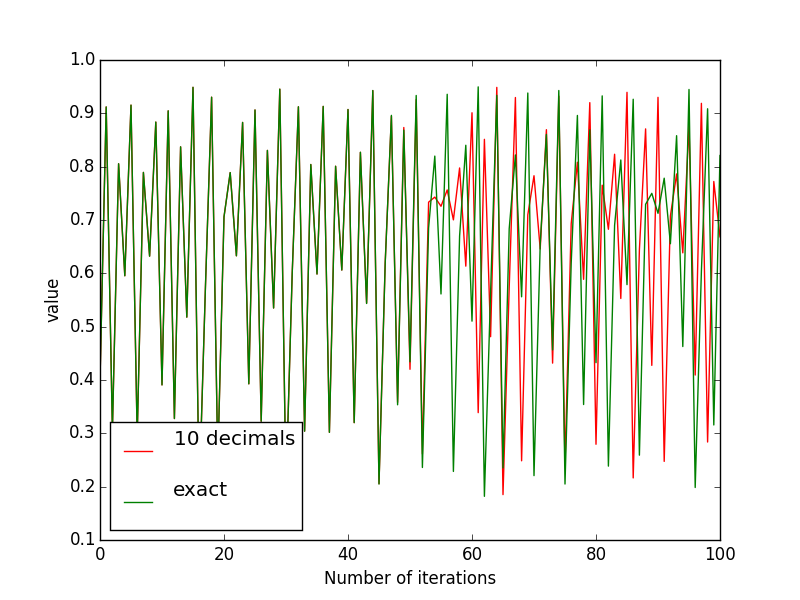
\includegraphics[width=0.5\textwidth]{img/dynamic_systems/logmap1}
    \caption{100 Iterations of the logistic map with $a=3.8$ and $x_0 = 0.4$ computed with 10 decimals precision and exactly.}
    \end{figure}
    \begin{figure}\label{fig:logmapprec}
    \centering
    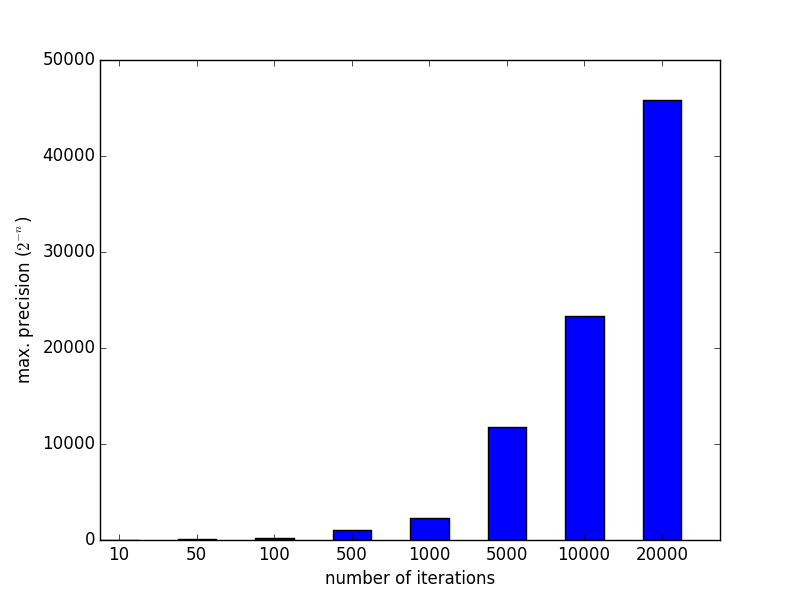
\includegraphics[width=0.5\textwidth]{img/dynamic_systems/logmap2}
    \caption{Maximal precision iRRAM uses to compute iterations of the logistic map and output the points with 10 decimal digits.}
  \end{figure}
  \subsubsection{The Shadowing Lemma}
    The term pseudo-orbit is used to describe numerically generated noisy orbits. 
    \begin{definition}\label{def:pseudoorbit}
      A sequence $(x_i)$ is called an \textbf{$\alpha$-pseudo-orbit} for a map $f$ if
      $ \| x_{i+1} - f(x_i) \| < \alpha $  
    \end{definition}
    One can think of a pseudo orbit as a numerically computed orbit, where small rounding errors can occur in every evaluation of $f$.
    \begin{definition}\label{def:shadowing}
      A real orbit $(y_i)$ \textbf{$\beta$-shadows} the pseudo-orbit $(x_i)$ if 
      $\| x_i - y_i \| < \beta$.  
    \end{definition}
    \begin{definition}
      A dynamic system is called \textbf{uniformly hyperbolic} if ...
    \end{definition}
    For systems that are uniformly hyperbolic Anosov and Bowen could show the following result \cite{anosov1967} \cite{Bowen1975} \cite{Hasselblatt:2008}:
    \begin{theorem}[Shadowing Lemma]
     For all $\beta > 0$ there exists an $\alpha > 0$ so that for every $\alpha$-pseudo-orbit $(x_i)$ there is a point $y_0$ so that the real orbit starting at $y_0$ $\beta$-shadows $(x_i)$.
    \end{theorem} 
    The logistic map is not hyperbolic...\\
    So for non-hyperbolic $f$, it can not be expected, that there is a real orbit that stays close to the pseudo orbit forever.
    Instead, there will be an orbit staying close to $(x_i)$ for some time, say up to some point $n_0$, and then starting to diverge. 
    The goal of this the case study is to investigate such orbits, in particular to find out how long there is an orbit staying close to the pseudo orbit,
    The basis for this case study is a paper by Hammel, Yorke and Grebogi from 1987 \cite{Hammel1987}.
    The paper deals with the question, how long numerical orbits of the logitstic map can be shadowed by true orbits.
    The authors show that for $a = 3.8$ and $x_0 = 0.4$, there is a true orbit $(y_n)$ of the logistic map, so that $\| x_n - y_n \| < 10^{-7}$ for $n \leq 10^7$.
    Their proof method is to compute bounds on the points of the true orbit by using a form of interval arithmetic and letting a computer do the computations. 
    All their computations are done on a Cray X-MP supercomputer. 
    For the case study, first their algorithm was implemented on a modern computer in the \cc programming language, both using fixed precision floating point numbers and \irram. 
    As a second step \irram was used to compute the shadowing orbit exactly.
  \subsubsection{The algorithm}
    The goal of the algorithm is to compute a shadowing orbit $(y_n)$ of size $N$ for a pseudo orbit $(x_n)$ of the logistic map $f$.
    Instead of computing the shadowing orbit from the first point, the algorithm computes the inverse orbit by starting with the last point and then iteratively computing the predecessor. 
    Since the logistic map is not injective, there is not a unique choice for this predecessor. 
    For some point $f(x)$ there are normally two possible values for the inverse given by $f^{-1}_{1,2}(x) = 0.5 \pm \sqrt{0.25 + \frac{x}{a}} $.
    An orbit can be computed by setting $y_N = x_N$ and then iteratively applying one of the inverse map $y_{n-1} = f^{-1}(y_n)$.   To stay close to the pseudo orbit, in every step the point on the same side of $0.5$ as $x_n$ is chosen (the index of $f^{-1}$ will from now on be omitted). 
    This works since the inverse function on $(0,1)$ is a contraction, thus
    $$ \| x_{n-1} - y_{n-1} \| = \| x_{n-1} - f^{-1}(y_n) \| \leq \| f^{-1}(x_n) - f^{-1}{y_n} \| + \| f^{-1}(x_n) - x_{n-1} \| \leq \| x_n - y_n \| + \delta $$   
    Since the original work had to do all the computations using floating point arithmetics, the inverse could not be computed exactly.
    Instead of the points $y_n$, a sequence of intervals $(I_n)$ that bound the location of $y_n$ is computed, i.e. so that $y_n \in I_n \text{ for } 0 \leq n \leq N$.
    The procedure is started with $I_N := [x_n, x_n]$ and then $I_{n-1}$ is selected so that $I_n \subseteq f(I_{n-1})$ holds and $I_n$ is chosen as small as possible. 
    Then the maximal distance between all points in $I_n$ and $x_n$ is computed.
    This gives a shadowing bound.
    An alternative to this algorithm, that instead computes the orbit in forward direction can be found in \cite{chow1991}.
\subsection{Implementation}
  The first part of the case study was to simulate the computations that were made on the Cray X-MP supercomputer on a modern computer. 
  The cray double precision data type used for the computations in the paper has machine epsilon $\varepsilon_\mu = 2^{-95}$.
  To compute the intervals $I_n$ from $I_{n+1}$ the inverse of the interval is computed as described above (using floating point arithmetic).
  Then as long as $I_{n+1} \not \subseteq f(I_n)$, $I_n$ is enlarged on both sides by the minimal possible quantity $\varepsilon_\mu$. 
  Since also the computation of $f(I_n)$ is done using floating point arithmetics, the condition might still not be fulfilled.
  This can, however, be compensated by further enlargening the interval on both sides by the constant $10^{-25}$.
  Since the precision of the clay double data type differs from the IEEE double precision, it was not possible using \cc's built in data types for simulating the algorithm.
  Instead, the boost multiprecision library \cite{boostmultiprecision} was used. 
  The library provides data types that replace the native \cc floating point types, but with a user defined precision. 
  For the interval arithmetic an interval class was implemented, having the following methods:\\
  CLASS DIAGRAM \\
  The same algorithm was also implemented in a different way. 
  Instead of using intervals with fixed precision floating point end points, \irram's \code(INTERVAL) type can be used. 
  The data type provides interval arithmetic for intervals with real numbered end points.
  Then, the inverse of an interval can be computed exactly.
  The next step, was to compute the shadowing orbit exactly.
  For that, only the pseudo orbit was calculated using floating point arithmetics. 
  Then, starting with the last point of the pseudo orbit the inverse was conputed exactly and the distance to the corresponding point in the pseudo orbit calculated.
  The maximum of all those distances is the distance of the shadow orbit and the pseudo orbit.
  One has to be a little careful though, when computing this maximum, since comparing two real numbers is not computable. 
  This problem can, however, easily be solved by the use of multi valued functions. 
\subsection{Evaluation}
  \subsubsection{Comparison with original work}
  The original work mainly deals with the case $a=3.8$ and $x_0 = $.

  Shadowing bound for different parameters
  Breaking point for different precisions
  Real orbit?

  %!TEX root = ../../thesis.tex
	Acknowledgment: Florian, Akitoshi
	\section{Introduction}
		In Chapter \ref{section:real_complexity} it was shown many important operators 
		on real functions are known to be computationally hard.

		On the other hand, for many of those functions, fast numerical algorithms working with 
    floating point arithmetic exist and are often very precise and reliable.

    Thus, there is a kind of mismatch between the worst case results in Computable Analysis
    and the practice of Numerical Analysis. 

    The following questions arise
		\begin{enumerate}
			\item What kind of functions are important and naturally arise in numerical analysis? 
			\item What kind of implicit assumptions are made about the functions and in what way do they allow faster computations? 
		\end{enumerate}

    Thus, it might be useful to consider subsets of real functions and investigate which of the operations become feasible.

		A subset of real functions that has been thoroughly studied in computable analysis are the analytic functions.
    It could be shown that many operators that are hard in the general case become polynomial time computable when restricting 
    to analytic functions.
     
    Note, however, that being analytic is a quite strong restriction on a function and that many problems in 
    numerical analysis deal with non-analytic functions.

    An analytic function is locally defined by its Taylor series, that is
		\begin{definition}
			For $z \in \CC$ and $r \in \RR, \, r > 0$, let $B(z,r) := \{ x \in \CC \,\, | x - z | < r\}$. \\
			A function $f: D \to \CC$ with $D \subseteq \CC$ is called \textbf{analytic}, if for every $x_0 \in D$ 
			the function given by the Taylor-series around $x_0$ converges to $f(x)$ for every $x$ in a neighborhood of 
			$x_0$. 

			That is, for every $x_0 \in D$ there is an $\varepsilon > 0$, such that for all $x \in B(x_0, \varepsilon)$ and there is a series
			$$ T(x) := \sum_{n=0}^{\infty} a_n(x-x_0)^n$$
			such that $T(x) \rightarrow f(x)$.

		\end{definition}
		The above definition can also be generalized to higher dimension. \\
		If $f$ is analytic then all its derivatives $f^{(n)}(x)$ exist and it holds
		$$ a_n = \frac{f^{(n)}(x_0)}{n!}. $$    

		The set of functions analytic on $D$ will be denoted by $C^\infty(D)$. \\		
		For the sake of simplicity, it will w.l.o.g. be assumed that $0 \in D$ and $x_0 = 0$ if not stated otherwise.
		
		Below are some properties of analytic functions.\\
    More detailed information on analytic function can for example be found in \cite{krantz2002primer}. 

		\begin{enumerate}
			\item For $f,g \in C^\infty(D)$ the sum  $f+g$ and the product $fg$ are analytic functions.
			\item If $f, g$ are analytic and $im(f) \subseteq dom(g)$ then their composition $f \circ g$ is analytic.
			\item The roots of an analytic function that is not identical to $0$ are isolated points.
			\item The derivative and anti-derivative of an analytic function are analytic.
			\item If the domain is connected, an analytic function is uniquely defined by a single Taylor-series around one point in its domain.
		\end{enumerate}

    The next theorem shows, that the property of being analytic is very useful when it comes to computability and complexity considerations.

    \begin{theorem}[Pour-El, Richards, Ko, Friedman \cite{pour1989computability}]\label{theorem:computable equiv series computable} 
			The following are equivalent
			\begin{enumerate}
				\item $f$ is computable 
				\item The series $(a_n)_{n \in \NN}$ is computable. 
 			\end{enumerate}
		\end{theorem}
    \begin{theorem}[M\"uller \cite{mueller1987uniform}]\label{theorem:computable equiv series computable polytime}
			The equivalence in Theorem \ref{theorem:computable equiv series computable} also holds, when the word computable is replaced by polynomial time computable.
		\end{theorem}
		
    Many operations on functions, like addition, multiplication, differentiation or anti-differentiation, can 
    be reduced to simple manipulations on the Taylor-series for analytic function.

		Thus, a direct consequence of Theorem \ref{theorem:computable equiv series computable polytime} is the following
		\begin{corollary}
			If $f \in C^\omega(D)$ is polynomial time computable the following functions are also polynomial time computable:
			\begin{enumerate}
        \item The functions obtained by the sum, product or difference of the two functions
				\item $i: D \to \RR$, $i(x) = \int_0^x f(t) dt$
				\item $d: D \to \RR$, $d(x) = f'(x)$ 
			\end{enumerate}
		\end{corollary}
		
		The above theorems show that computing with analytic functions is in some sense much easier than the general case.

		However, those theorems are non-uniform in the following sense:

		The theorems only say that, that $f$ being polynomial time computable implies the existence of a polynomial time computable sequence
		and the existence of such a sequence implies that there exists some algorithm computing $f$ in polynomial time. \\
		In no way, however, do they say, how to compute the sequence from a given representation of the function and vice versa.

		In fact the following theorems show, that this is not a problem of those theorems, but it's inherently impossible to do so.
		\begin{theorem}[M\"uller \cite{mueller1987uniform}]
			Let $f$ given as in Definition \ref{def:representation} then the operator $f \to (a_n)_{n \in \NN}$ computing the Taylor series around $0$ (or any other point) is not computable.
		\end{theorem} 
		\begin{theorem}[M\"uller \cite{mueller1987uniform}]\label{theorem: evaluation not uniformly computable from powerseries}
			Let $(a_n)_{n \in \NN}$ be the series expansion around $0$ for some $f \in C^\omega(D)$.\\
			The evaluation operator $((a_n)_{n \in \NN}, x) \to f(x)$ that, given a series and a point, computes the value of the corresponding function at that point, is not computable.
		\end{theorem} 

		The reason for the non-uniformity is, that any algorithm can only read a finite number of 
		coefficients from the series. But from the power series alone, it is impossible to know how many coefficients are needed to make
		a good enough approximation. This information can not be (computably) extracted from the Taylor-series, thus the algorithms have to 
    be given some additional information.

		The goal of this case study was to write a general data type for analytic functions. 
		Due to the above any such data type will need more information than only the series of Taylor coefficients. \\
		The next section will deal with the question, what additional information is needed to get uniform versions of the above theorems.

	\section{Representation of Analytic Functions}
	 As seen in the previous section, the information given by the series expansion is not enough to make reasonable computations with analytic functions.
	 However, by enriching the information by some finite discrete parameters, the translation between Taylor-series and function representation can be made uniform 
   and even polynomial time computable.
	 
	 Two possible representations for analytic functions on the closed unit disc are as follows
	 \begin{definition}\label{def:series_name_ball}
	 	A \textbf{series-name} $\rho_s$ of $f \in C^\omega(\overline{B_1(0)})$ is a triple $((a_n)_{n \in \NN}, k, A)$ where 
	 	\begin{enumerate}
	 		\item $(a_n)_{n \in \NN}$ is the series expansion of $f$ around $0$
	 		\item $\sqrt[k]{2} \leq R$ 
	 		\item $|a_j|r^j \leq A$ for all $j \in \NN$
	 	\end{enumerate}
	 	and $R = (\limsup |a_j|^{\frac{1}{j}})^{-1}$ denotes the radius of convergence of the series.
	 \end{definition}
	 The two additional parameters are useful, because they can be used to make a tail estimate 
	 \begin{equation}\label{eqn:tail_estimate}
	  \left | \sum_{n \geq N} a_nx^n \right | \leq A \frac{(|z|/r)^N}{1-|z|/r}
	 \end{equation}
	 A name as in Definition \ref{def:series_name_ball} can be found by choosing any appropriate $k$ (note that the radius of convergence is always bigger than $1$) and choosing $A$ as an upper bound of $f$ extended to $\overline{B_{\sqrt[k]{2}}(0)}$. 
	 \begin{definition}\label{def: function name ball}
	 	A \textbf{function-name} $\rho_f$ of $f \in C^\omega(\overline{B_1(0)})$ is a triple $(f, l, B)$ such that
		B is an upper bound of $f$ on $\overline{B_{\sqrt[l]{2}}(0)}$.
	 \end{definition}
	 \begin{theorem}\cite{Kawamura}\label{thm:representation_conversion}
	 	The mapping between $\rho_s$-name and $\rho_f$-names is computable in time polynomial in 
	 	$n+k+\log(A)$ and the inverse mapping is computable in time polynomial in $n+l+\log(B)$ 
	 \end{theorem}
	 Note that the above translation becomes fully polynomial time when in the representations $k$ resp. $l$ are required to be encoded in unary, while $A$ resp. $B$ are given in binary.
	 Thus, from now on the term polynomial time computable will be used when referring to running time bounds as in Theorem \ref{thm:representation_conversion}.

	 A full proof of Theorem \ref{thm:representation_conversion} can be found in \cite{Kawamura}. 

   Some details that are important for the implementation are given below as seperate theorems.

   \begin{theorem}
     A series name can be used to evaluate the corresponding function in polynomial time.
     \begin{proof}
       According to Equation \ref{eqn:tail_estimate} if the first $N := nk+\log A$ terms are summed up then the error 
       $$ \left | \sum_{j > N} a_j r^j \right | \leq 2^{-n} $$
     \end{proof}
   \end{theorem}

   \begin{theorem}
    Given a function name it is possible to compute any Taylor coefficient $a_n$ around $0$ of the function
    in polynomial time.
    
	 \begin{proof}
	 	To compute a series name from a function name, one has to compute the coefficients of the series 
    expansion from a function name, i.e. from the function and the parameters $l$ and $B$.

	 	In \cite{Muller1993} M\"uller describes an algorithm for this task.
	 	To approximate the coefficient $a_k$ with precision at least $2^{-n}$ $f$ is approximated by the Lagrangian interpolation
	 	polynomial
	 	\begin{equation}\label{eqn:interpolation_polynomial}
	 		P_m(x)  :=  \sum_{i=0}^{2m} f(x_i) \cdot L_{m,i}(x) 
	 	\end{equation}
	 	where
	 	\begin{eqnarray*}
	 		x_i & = & (i-m) \cdot h , h \in \RR, h > 0 \\
	 		L_{m,i}(x) & = & \prod_{i \neq j} \frac{x-x_j}{x_i-x_j} 
	 	\end{eqnarray*}
	 	Differentiating Equation \ref{eqn:interpolation_polynomial} $k$ times yields
	 	\begin{equation}\label{eqn:interpolation_polynomial_diff}
	 		P_m^k(0)  :=  \sum_{i=0}^{2m} f(x_i) \cdot L_{m,i}^{(k)}(0) 
	 	\end{equation}
	 	Let $\sigma = \lceil \log_2 B \rceil + 1$

	 	It can then be shown that if $f$ is evaluated on $2k+1$ points from the 
	 	real interval $\{x \in \R \,|\, |x| \leq \frac{1}{2}\}$ with precision $2n+15k+\sigma+6$ 
	 	then $a_k$ can be approximated by the above procedure with error less than $2^{-n}$ in 
	 	$O((k+1)\cdot \M(n+k+\sigma) + k^2 \M (k \log k)$

    The coefficients $L_{m,i}^{(k)}(0) $ in Equation \ref{eqn:interpolation_polynomial_diff} 
    are rational numbers and can be computed by a recursion formula.
	 \end{proof}
   \end{theorem}

	 \begin{theorem}\label{thm:polytime_on_ball}
	 	The following is polynomial time computable when given $\rho_s$ or $\rho_f$ names for the input functions.
	 	\begin{enumerate}
	 		\item Evaluation $(f,z) \to f(z)$
	 		\item Addition $(f_1, f_2) \to f_1 + f_2$
	 		\item Multiplication $(f_1, f_2) \to f_1 \cdot f_2$
	 		\item $d$-fold Differentiation $(f,d) \to f^{(d)}$ where $d$ is given as unary
	 		\item $d$-fold Anti-differentiation $(f,d) \to \int \dots \int f$ where $d$ is given in unary
	 	\end{enumerate}
    \begin{proofsketch}
	 		Evaluation follows from \ref{thm:representation_conversion}. \\
	 		The manipulations that have to be done on the Taylor series are straight forward, 
      e.g. addition can be done by just adding the coefficients of the two series.
      
	 		It remains to show how to compute the new parameters $A'$ and $k'$ from the parameters $A_1, A_2, k_1, k_2$. 
      The results will just be listed here without proof.
      \begin{enumerate}
        \item Addition: $A' = A_1 + A_2$ and $k' = max(k_1, k_2)$.
        \item Multiplication: $k' = 2\max(k_1, k_2)$ and $A'$ is some integer such that $A' \geq A_1 \cdot A_2 \cdot (1 + \frac{k'}{e \ln 2})$.
        \item Differentiation: $k' = 2k$ and $A'$ is some integer such that $A' \geq \frac{A}{r} \cdot (1+\frac{2k}{e\ln 2})$.
          Note, that the parameters do not depend on $d$.
        \item Anti-Differentiation: $k' = k$ and $A'$ an integer such that $A' \geq A \cdot r^d$.
      \end{enumerate}
	 	\end{proofsketch}
	 \end{theorem}

	The above can be extended to a data type for analytic functions on arbitrary ball-shaped domains.\\
	But of course, most domains are not ball-shaped and one would also like to represent such domains.
	
	One possible way to represent functions on such a domain, is to cover the domain with balls and use the representation from Definition \ref{def:series_name_ball} on each ball.
	As an example, consider functions analytic on the real line $[-1,1]$ (this implies being analytic on a rectangle around the line $[-1,1]$ in the complex plane).
	

	 \begin{figure}
	 	\centering
	 	\begin{subfigure}{.45\textwidth}
	 		\centering
			\begin{tikzpicture}[scale=0.8]
			    \node  at (-0.2,-0.5) {$-1$};
			    \node  at (4.0,-0.5) {$1$};
			    \draw [thick,|-|] (0,0) -- (4,0);
			    \node  at (1.5,.6) {$\frac 1{2k}$};
			    \draw  [dotted] (2.0,0) -- (2.0,1);
			    \draw [domain = 0:8,color=gray] plot[samples=160] (\x-2, {sqrt(16-(\x-4)^2)*(1-1/(\x^2+1) + sin(\x) + (\x/7)^5-\x/6 +1.5- 1/((\x-5)^2+1))/2});
			    \draw [domain = 0:8,color=gray] plot[samples=160] (\x-2, {1/(\x^2+1)/2 + sin(80*\x) + (\x/7)^5-\x/6 -1-sqrt(16-(\x-4)^2)/2});
			    \draw [color=gray] (-2,0) -- (-2,-.5);
			    \draw [color=gray] (6,.19) -- (6,-1.42);
			    \node [color=gray] at (.5,2) {$dom(f)$};
			    \draw [fill=blue,radius =.05,color=blue] (3.5,0) circle;
			    \node [color=blue] at (3.5,-.2) {$x_0$};
			    \draw [fill=blue,radius =.05,color=blue] (2.0,0) circle;
			    \node [color=blue] at (2.0,-.2) {$x_1$};
			    \draw [radius = 1,color=blue, dotted] (2.0,0) circle; 
			    \draw [fill=blue,radius =.05,color=blue] (0.5,0) circle;
			    \node [color=blue] at (0.5,-.2) {$x_2$}; 
			    \draw [radius = 1,color=blue, dotted] (0.5,0) circle;
			    \draw [radius = 1,color=blue, dotted] (3.5,0) circle;
			    \draw [radius = 1.8, color = red, dotted] (3.5,0) circle; 
			    \draw [fill=red,radius = .05,color = red] (3,1.75) circle;
			    \node [color=red] at (3,1.45) {$singularity$};
			\end{tikzpicture}
			\caption{For a series name the domain is covered with equally sized balls. 
			For each ball a Taylor series around the center of the ball is given and the properties of Definition \ref{def:series_name_ball} hold.}\label{fig: analytic function representation series name}
		\end{subfigure}
		\centering
	 	\begin{subfigure}{.45\textwidth}
			\begin{tikzpicture}[scale=0.8]
			    \draw (-1,1) rectangle (5,-1);
			    \node  at (-0.2,-0.5) {$-1$};
			    \node  at (4.0,-0.5) {$1$};
			    \draw [thick,|-|] (0,0) -- (4,0);
			    \node  at (-.7,-.25) {$\frac 1l$};
			    \draw  [dotted] (-1,0) -- (0,0);
			    \node  at (2.2,.5) {$\frac 1l$};
			    \draw  [dotted] (2,1) -- (2,0);
			    \node  at (-.5,0.6) {$\overline R_l$};
			    \draw [domain = 0:8,color=gray] plot[samples=160] (\x-2, {sqrt(16-(\x-4)^2)*(1-1/(\x^2+1) + sin(\x) + (\x/7)^5-\x/6 +1.5- 1/((\x-5)^2+1))/2});
			    \draw [domain = 0:8,color=gray] plot[samples=160] (\x-2, {1/(\x^2+1)/2 + sin(80*\x) + (\x/7)^5-\x/6 -1-sqrt(16-(\x-4)^2)/2});
			    \draw [color=gray] (-2,0) -- (-2,-.5);
			    \draw [color=gray] (6,.19) -- (6,-1.42);
			    \node [color=gray] at (.5,2) {$dom(f)$};
			    \draw [fill=red,radius = .05,color = red] (3,1.75) circle;
			    \node [color=red] at (3,1.45) {$singularity$};
			    %\draw [radius = 1, color = blue, dotted] (2.5,0) circle;
			    %\draw [fill=blue, radius = .05, color = blue] (2.5,0) circle;
			    %\node [color=blue] at (2.5,-.2) {$x_1$};
			\end{tikzpicture}
			\caption{A function name encodes a closed rectangle around $[-1,1]$ where the function is analytic and an upper bound for the function on that rectangle.}\label{fig: analytic function representation function name}
		\end{subfigure}
		\caption{Representations for functions analytic on the real line $[-1,1]$}\label{fig: analytic function representations}
	 \end{figure}
	\begin{definition}\label{def:series_name_rect}
		Let $f \in C^\omega([-1,1])$.
		A \textbf{series-name} for $f$ is a 5-tuple $(M, (x_m), (a_{n, j}), k, A)$ where $M \in \NN$
		$1 \leq j \leq M$, $n \in \NN$, $x_m \in [-1,1]$ and it holds
		\begin{enumerate}
			\item $[-1,1] \subseteq \bigcup_{m=1}^M [x_m - \frac{i}{4k}, x_m + \frac{1}{4k}]$
			\item $(a_{n,i})_{n \in \NN}$ is the series expansion of $f$ around $x_i$
			\item $|a_{n,i}| \leq Ak^n$ for all $n \in N$, $1 \leq i \leq M$
		\end{enumerate}
	\end{definition}
	To simplify the definition the parameters $k$ and $A$ were chosen global, i.e. they hold for each of the series.
	That means, the domain is covered by equally sized balls. 
	Figure \ref{fig: analytic function representation series name} shows a series name with three series.
	
	The definition can be further simplified by requiring the series centers to be equidistantly distributed on $[-1,1]$ and thus
	making it unnecessary to store them in the representation.

	A function name as in Definition \ref{def: function name ball} can also be defined
	\begin{definition}
		Let $R_l := [-\frac{1}{l}, 1+\frac{1}{l}] \times [-\frac{1}{l}, \frac{1}{l}]$ the closed rectangle with distance $\frac{1}{l}$ around $[-1,1]$ .\\
		A \textbf{function-name} for a function $f \in C^\omega([-1,1])$ is a 3-tuple $(f|_{[-1,1]}, B, l)$ with $B, l \in \NN$ such that 
		\begin{enumerate}
			\item $f \in C^\omega(R_l)$
			\item $B$ is an upper bound for $f$ on $R_l$
		\end{enumerate}
		where $l$ is coded in unary and $B$ in binary.
	\end{definition}
	See Figure \ref{fig: analytic function representation function name} for a picture describing the function name. 

	Again it can be shown that the two representations are polynomial time equivalent, and that the equivalent to
	Theorem \ref{thm:polytime_on_ball} holds.
	\section{Analytic Continuation}
		One problem with the representation in Definition \ref{def:series_name_rect} is that when thinking of this representation as an interface for a data type, it is very cumbersome for the user to provide all the information needed. 
		He would need to give an algorithm for as many Taylor series as needed to cover the interval.
		\begin{figure}
			\centering
			\begin{tikzpicture}[scale=1.6]
			    \draw (-1,1) rectangle (5,-1);
			    \draw [thick,|-|] (0,0) -- (4,0);
			    \node at (-.5,-.25) {$\frac 1l$};
			    \draw [dotted] (-1,0) -- (0,0);
			    \node at (2.2,.5) {$\frac 1l$};
			    \draw [dotted] (2,1) -- (2,0);
			    \draw [fill=blue,radius =.05,color=blue] (3.5,0) circle;
			    \node [color=blue] at (3.5,-.2) {$x_0$};
			    \draw [radius = 1,color=blue] (3.5,0) circle;
			    \draw [fill=green, radius = .05, color = green] (1.5,0) circle;
			    \node [color=green] at (1.5,-.2) {$x$};
			    \draw [fill=cyan, radius = .05, color = cyan] (2.75,0) circle;
			    \node [color=cyan] at (2.75,-.2) {$x_1$};
			    \draw [radius = 1,color=cyan] (2.75,0) circle;
			    \draw [fill=blue, radius = .05, color = blue] (2.25,0) circle;
			    \node [color=blue] at (2.25,-.2) {$x_2$};
			    \draw [radius = 1,color=blue] (2.25,0) circle;
			\end{tikzpicture}
			\caption{Evaluation by Analytic Continuation: 
					to evaluate the function at point $x$ given the series around $x_0$, first the series around 
					point $x_1$ is computed. This series is used to compute one more series around $x_2$ which then finally
					can be evaluated at $x$.}\label{fig: analytic continuation}
		\end{figure}

		As said before, there is no real gain of information by providing all those series.
		The analytic function is uniquely defined by the Taylor series around a single point.

    A simplified representation can therefore be as follows
		\begin{definition}
			A \textbf{single series name} for $f \in C^\omega([-1,1])$ is a quadruple $(x_0, (a_n)_{n \in \NN}, k, A)$ such that
			\begin{enumerate}
				\item $(a_n)_{n \in \NN}$ is the series expansion of $x$ around $x_0$
				\item $A$ and $k$ are such that $| a_m | \leq Ak^m$ 
			\end{enumerate}
		\end{definition}
		A series name can be obtained from a single series name by computing the series expansion on another point on the domain and then iterating this process until the series cover $[-1,1]$.

		Since the parameters $A$ and $k$ are such that they hold on the entire rectangle, 
		the new series will be valid on a ball with the same radius as the original series, effectively extending the domain.
		This process is called \textbf{analytic continuation},
		
		The series can be computed either by applying the algorithm from the proof of Theorem \ref{thm:representation_conversion} or by directly computing the derivatives at an other point using Theorem \ref{thm:polytime_on_ball}.
		Note however, that iterating this process will break the polynomial time computability, as will be shown in the next
		section.
	\section{Complexity Analysis}
		The previous section gave an overview of the representations and how they can be used to yield efficient 
    (in the sense of polynomial time computability)	operations on analytic functions.
		Since for practical applications polynomial time computability is too coarse a measure for efficiency, 
		in this section a more refined analysis on the algorithms is done. 

		The goal is to establish time bounds in terms of the $O$-notation.
		
		Most of this has already been done in \cite{mypaper}, thus proofs are omitted or only sketched.

		Let $T(a_m, n)$ denote the running time needed to compute the coefficient $a_m$ from the Taylor series with an error 
		less than $2^{-n}$.
		The running time of all operations on the Taylor series will depend on this factor.

		Let further denote $\M(n)$ the time needed to multiply two $n$-bit numbers (e.g. $\M(n) = O(n\log n \log \log n)$ when using the Schoenhage-Strassen Algorithm \cite{Schonhage1971}). 		
		\begin{theorem}
			Given a series name of $f \in C^\omega(D)$.
			To evaluate $f$ with error less than $2^{-n}$ 
			$$N = k(n+\lceil log_2(log_2 (e^2) kA \rceil)$$
			coefficients of the Taylor series are sufficient. \\
			This yields evaluation computable in time 
			$$ O(N\M(N)+N \cdot T(a_N, n+log_2(N)+1)) $$ 
		\end{theorem}

		\begin{theorem}
			The $m$-th coefficient of the $d$-times differentiated series is given by $a_m^{(d)} = a_{m+d} \prod_{i=1}^d (i+m)$.
			
			Computing the $m$-th coefficient of the series for the $d$-fold derivative can thus be done
			$$ O(T(a_{m+d}, n+d\log_2(d+m)))+d\M(d \log_2 (d+m)+n)) $$
		\end{theorem}

		\begin{theorem}
			Given a series name of $f \in C^\omega(D)$, the number of coefficients of the series of the $d$-fold derivative computed from $f$ as in Theorem \ref{thm:polytime_on_ball} needed to evaluate this derivative, is given by 
			$$N_d = k\left(n+\lceil log_2(log_2 (e^4) kA \rceil+\left \lceil d\left(\log_2(d)+\log_2(\log_2(e)k+1)-\frac{1}{k}\right)\right\rceil\right).$$
			Thus, evaluating the $d$-fold derivative of $f$ is possible in time bound by
			$$ O(N_d\M(N_d)+N_d \cdot T(a_{N_d+d}, n+d\log_2(d+N_d)))+d\M(d \log_2 (d+N_d)+n) $$ 
		\end{theorem}
		For computing the $m$-th coefficient of a Taylor series around some point the $m$-th derivative 
		has to be divided by $m!$. This division reduces the needed precision leading to 
		$$N_{coeff}(m) = 2k\left( n+\lceil log_2(\log_2 (e^4) kA) + m \log_2(log_2(e)k+1)\rceil \right)$$
		as the number of coefficients that are needed to compute the $m$-th coefficients of the Taylor series 
		around another point. 
    
		For stepwise analytic continuation it is necessary to iterate the process of differentiating.
		For example, using the single series name when one wants to evaluate the function at a point $x$
		that is not inside the ball of the given series, analytic continuation has to be applied until a series
		containing $x$ is reached.

		Assume for a computation the coefficients up to $N$ of the last series is needed. 
		The previous results lead to the recurrence relation
		relation 
		\begin{eqnarray*}
			N^{(0)} &=& N \\
			N^{(l+1)} &=& 2k\left( n+\lceil log_2(\log_2 (e^4) kA) + N^{(l)} \log_2(log_2(e)k+1)\rceil \right)
		\end{eqnarray*}
		further leading to
		\begin{theorem}
			Applying analytic continuation $l$ times, to compute $N$ coefficients of the last series 
			\begin{equation}
				N^{(l)} = O((2k \log_2 (\log_2 (e)k +1))^lN) 
			\end{equation}
			coefficients of the original series are needed.
		\end{theorem}
		The above leads to a running bound for evaluating using $l$-times iterated analytic continuation.
		\begin{theorem}
			The running time of evaluating the $l$ times iterated series is bounded by
			\begin{equation}
				 O(l(N^{(l)})^2\M(N^{(l)})+N^{(l)}T(a_{N(l)}, l N^{(l)}\log_2(N^{(l)}))) 
			\end{equation}
		\end{theorem}
		Due to the number of parameters the running time depends on, the above bounds are quite complicated.\\
		To get get simple bounds the following assumptions were made
		\begin{enumerate}
			\item $A$ and $k$ are usually very small compared to the other parameters, 
			thus they are neglected except for the case when $k$ is in the base of an exponentiation.
			\item The time $T(a_m, n)$ to read a coefficient of the series is neglected. 
			Although this time has a huge impact on the overall running time, for reasonably fast sequences it 
			the time will be dominated by the other parameters.
		\end{enumerate}
		This leads to the following simplified bounds
		\begin{enumerate}
			\item Evaluation of a series-name is possible in time $O(n\M(n))$.
			\item Evaluation of the $d$-fold (anti-)derivative is possible in time $O((n+d)\M(n+d))$
			\item Evaluation of the $l$ times iterated analytic continuation is possible in time $O((2k \log k)^{2l}n^2\M((2k\log k)^ln)$
			\item The number of coefficients that have to be read from the original series to evaluate a series gained by 
			$l$-times iterated analytic continuation is bound by $O((2\log_2(\log_2(e)+1))^l) = O(2.56^l)$
		\end{enumerate}

	\section{Implementation}
		\irram was used as a framework to implement the ideas in the previous section.
		The goal was to add user friendly classes for analytic functions to \irram.
		In particular two classes were created for this purpose.

		The class \baana is a basic class for analytic functions on 
		a closed disc with rational radius around $0$, inspired by Definition \ref{def:series_name_ball}.

		The class \anarect is a class for functions analytic on an arbitrary real interval $[a,b]$, 
		inspired by Definitions \ref{def:series_name_ball} and \ref{def:series_name_rect}.

		Both classes provide a common set of operators and methods, in particular
		\begin{enumerate}
			\item It is possible to add, multiply and subtract two objects using the overloaded operators $+$, $*$, $-$.
			\item It is possible to evaluate the function at $x \in D$ using the overloaded operator $()$
			\item There is a function \code{differentiate (unsigned int n)} to get a new object representing the $d$-th derivative of the analytic function.
			\item There is a function \code{integrate (unsigned int n)} to get a new object representing the $d$-th anti-derivative of the analytic function.
			\item It is possible to get the coefficients of the underlying Taylor series.
		\end{enumerate}

    Since a power series is an infinite object, some thought has to be put into how to represent it on a computer.

    Some reasonable approaches are for example
		\begin{enumerate}
			\item A finite representation, i.e. at every point of time during the execution of the program, 
			only a finite initial segment of the power series is known. 
			Thus, all computations are performed on polynomials. 
			The length of the initial segment depends on the desired precision and grows 
			with the iterations of \irram.
			\item A functional representation, i.e. a powerseries is a function from an integer $n$ to the coefficient
			$a_n$ (or a pointer to such a function). If a coefficient is needed it can be simply computed by calling the function.
		\end{enumerate}
		
		The second method is very similiar to the DAG approach and can therefore suffer from the same memory issues.
		Even tough this is true and also the first method is arguably more in the spirit of the \irram framework, a decision was made to follow the second approch.

		There are several reasons for that. Firstly, the number of coefficients needed from the power series depends heavily on the point where the analytic function is evaluated. 
		If the length of the used initial segment grows with the internal precision of \irram, worst case assumptions have to be 
		made on the needed number of coefficients. 
		This would in most cases be a huge overestimation and therefore lead to longer computation times.

		Secondly, the memory issue does not play such a big role in this case. 
		Usually, operations like derivation or analytic continuation, that increase the size of the DAG 
		are not applied hundred thousands of times, but orders of magnitude less. 
		Thus, the DAGs stay rather small and easily fit into the main memory of a modern computer.

		The pure functional approach, however, has the disadvantage that a coefficient has to
		be computed every time it is needed and thus the same work might have to be done many times. 
		Depending on the algorithm, this can lead to very poor performance.

		To prevent this, a form of caching was implemented. The coefficient function is only called the first time, when a 
		coefficient needs to be computed and then saved to the cache. The next time the coefficient is accesed it is taken from 
		the cache instead of calling the function again. 
    Thus the coefficient is only recomputed when the precision is not sufficent and \irram reiterates the computation.



	\section{Class Overview}
		In addition to the two classes for analytic functions, several helper classes were implemented.
    The design of the implementation is very close to the interface given by the theoretical framework, i.e.
    there are classes for different mathematical objects, that work on representation classes for that object.

		All classes were implemented with generic types using Templates, whenever it made sense.

		The following classes exist
		
		\subsection{\poly} 
			\textbf{\code{POLY<coeff\_type>}} is a class template for polynomials of a generic coefficient type. 
			The class for the coefficient type should have implementations of the \code{*} and \code{+} operators
			and it should be possible to cast $0$ to \code{<coeff\_type>}.

			The following has been implemented for \poly
			\begin{enumerate}
				\item Constructor from a \code{vector<coeff\_type>} and default constructor (constant zero polynomial).
				\item Copy constructor \code{POLY(const POLY<coeff\_type>\& P)} and Copy assignment constructor \code{POLY\& operator = (const POLY<coeff\_type>\& P)}.
				\item Methods \code{get\_degree()} and \code{get\_coeff(const unsigned int n)} returning the degree and a specific coefficient.
				\item Addition, Subtraction, Multiplication and Scalar Multiplication via the overloaded operators \code{+}, \code{-}, 	\code{*}, \code{+=}, \code{*=}.
				\item Evaluation via the overloaded operator \code{()}.
				\item symbolic differentiation and anti differentiation via the functions \code{void diff(unsigned int)} and \code{void integrate(unsigned int n)}.
				\item A function \code{void rwrite(const POLY<coeff\_type>\& P, int precision)} that outputs the polynomial
				in the form $a_n*X^n+ \dots a_n*X + a_0$ where the real numbers $a_0, \dots, a_n$ are written with the number of decimals given by the parameter \code{precision}.
			\end{enumerate}
			All methods were implemented in the most straight forward way. \temp{Evaluation should be Horner Scheme?}
		\subsection{\func}
			\textbf{\code{FUNC<RESULT(PARAM)>}} is a class template for functions with input 
			of type \code{PARAM} and return type \code{RESULT}. 
      It can be seen as a thin wrapper around \code{std::function}.
			
      The idea behind \func is to have a class for functions in the mathematical sense, thus the classes for the template
			parameters should have the arithmetical operators implemented.

			The following methods exists
			\begin{enumerate}
				\item Constructors from an \code{std::function} or a pointer an \code{std::function}.
				\item  Copy constructor \code{FUNC(const FUNC<RESULT(PARAM)>\&)} and copy assignment constructor 
						\code{FUNC\& operator = (const FUNC<RESULT(PARAM)>\&)}
				\item Addition, Subtraction, Multiplication and Scalar Multiplication via the overloaded operators \code{+}, \code{-}, 	\code{*}, \code{+=}, \code{*=}
				\item Evaluation with the operator \code{()}
				\item Function Composition with the operator \code{()}
			\end{enumerate}
			Methods are performed on a representation class called \code{rep\_rho\_D}.
      
      Straight forward implementations of all operations are possible using {\ccx}'s lambda functions, e.g. addition is implemented the following way
			\lstinputlisting{code/func_addition.cc}
		\subsection{\powerseries}
			\textbf{\code{POWERSERIES<coeff\_type>}} is a class template for power series of a generic coefficient type, 
			i.e. a (symbolic) series of the form $ \sum_{i=0}^\infty a_n \cdot x^n$.

			The same restrictions on the coefficient type as for \poly hold.
			
			The series itself is represented as a \code{FUNC<coeff\_type(unsigned\ int)>}, i.e. a function from the integers to \code{coeff\_type}.
      
      Note, that hereby the maximal number of coefficients is limited by the size of \code{unsigned int}, 
			but the limit is large enough to have no practical relevance.   

			\powerseries has the following methods
			\begin{enumerate}
				\item Constructors from a \code{shared\_ptr} to a \code{FUNC<coeff\_type(unsigned\ int)>} and from a single object of \code{coeff\_type} (giving a sequence with constant coefficient sequence).
				\item Copy constructor \code{POWERSERIES(const POWERSERIES<coeff\_type>\& P)} and copy assignment constructor 
				\code{POWERSERIES\& operator = (const POWERSERIES<coeff\_type>\& P)}.
				\item A method \code{coeff\_type get\_coeff(const unsigned int\& n)} returning the $n$-th coefficient
				\item A method \code{POLY<coeff\_type> cut\_of\_at(const unsigned int\& n)} that returns the polynomial given by 
				$ \sum_{i=0}^n a_i x^i $.

				\item Addition, Subtraction, Multiplication and Scalar Multiplication via the overloaded operators \code{+}, \code{-}, \code{*}, \code{+=}, \code{*=}
				\item symbolic differentiation \code{void differentiate(int n)} [where did anti differentiation go?]
				\item Composition of \powerseries using the operator \code{()}
			\end{enumerate}
			The methods are mainly implemented as realizer functions on the corresponding representation class \code{rep\_rho\_dy\_omega}. 

			Again, the implementation is mostly straight forward transformations on the power series. 

			Since the objects that are manipulated are functions {\ccx}'s functional features come in handy and are used heavily. 		

      This class also implements a form of caching for the power series coefficients.
      
      The \code{rep\_rho\_dy\_omega} class contains a \code{vector<coeff\_type>} and whenever
      a coefficient is read, all coefficients up to this one are saved in the \code{vector} and retrieved from there when read the next time.

	\subsection{\baana}
		\textbf{\code{BA\_ANA<ARG>}} is a class template for functions analytic on a closed disc with some rational radius $r$ around $0$. 

	  In the current form, for the template parameter \code{ARG} only \real or \complex makes sense. 
		
		Apart from the methods at the beginning of this section, the following methods exists
		\begin{enumerate}
			\item A constructor from a \powerseries, two \code{INTEGER}s $k$ and $A$ and a \code{RATIONAL} $r$.
			To work correctly $r$ has to be strictly smaller than the radius of convergence $R$ 
			and it has to hold $\sqrt[k]{2r} < R$ and $|a_n| \leq \frac{A}{r^n \cdot 2^{n/k}}$.
			\item A constructor from a \func, two \code{INTEGER}s $k$ and $A$ and a \code{RATIONAL} $r$.
			\item A method \code{POWERSERIES<ARG> series\_around(const ARG\&)} that computes the series expansion around
			an arbitrary point in the domain.
			\item Composition using the \code{()} operator.
		\end{enumerate}
		
		\baana uses two representation classes, \code{rep\_pi}, the representation by a power series, and \code{rep\_rho\_D\_refined}, the represention as a function. 
		All operations except evaluation use the power series representation. 
		If the constructor from a function object is called, the power series will also be computed, 
		thus the \code{rep\_pi}-name is always available.

		Evaluation can also be realized from the \code{rep\_pi} name, but it will usually be faster 
		to use the function if it is available.

    The methods are implemented as described in Theorems \ref{thm:polytime_on_ball} and \ref{thm:representation_conversion}. 

    For evaluation it is very useful to have access to {\irram}'s internal representation of the error of a \real. \\
    The value $f(x)$ is obtained summing up a finite initial segment of the Taylor series $ \sum a_i x^n $.

    The error consists of two parts, the error that is made because of the truncation (see \ref{eqn:tail_estimate}) and 
    the error that is made because of the coefficients and $x$ only being available as finite approximations. 
    
    While summing up the terms in the sum, the second type of error might become bigger than the first type.
    In that case, it is better to stop the summation and return a \real with a too big error, to make \irram start a new 
    iteration with more precise approximations to the coefficients and $x$.
   
	\subsection{\anarect}
		The class \anarect represents complex functions that are analytic on an interval $[a, b] \subseteq \RR$.
		The internal representation is very similiar to the one in Definition \ref{def:series_name_rect}.
		That is, a finite sequence of (overlapping) equidistant Taylor sequences covering the interval and parameters $A$ and $k$ 
		that are valid for all the series.

		Apart from the methods common with \baana the following exist
		\begin{enumerate}
      \item A constructor from (a pointer to) a \powerseries, the two integers $k$ and $A$ and two {\real}s \code{left} and \code{right}
            that give the end points of the line where the \anarect object will be defined.
      \item A constructor from a function pointer, two \code{INTEGER}s $l$ and $B$ and \code{left} and \code{right} as above.
      \item A method \code{get\_series\_number(int n)} that returns a pointer to the \powerseries for the $n$-th series.
      \item The method \code{cut\_of\_at(int n, int m)} returns a \poly with the first $m$ coefficients of series $n$. 
		\end{enumerate}
		The constructor only takes a single \powerseries.
		All other power series needed to cover the interval are computed from the provided one using analytic 
		continuation.  

		\anarect uses two representation, a function representation \code{rep\_fun} and a series representation \code{rep\_ana\_rect} that can be transformed into each other.

		The series representation \code{rep\_ana\_rect} contains a \code{vector} with the power series.
		When evaluating the \code{rep\_ana\_rect}-name at a point $x \in \CC$, 
		a Taylor series containing $x$ is chosen and then a \baana object of this series created and evaluated at 
		the (appropriately shifted) point $x$. 

		For other operations, the according transformation of the first series is computed and then the 
		other series are computed from that.    
	\section{Usage}
		The following \cc program gives an example how the \baana class can be used. 
    \anarect can be used similiarily.
    \lstinputlisting[numbers=left,stepnumber=1,firstnumber=1,numberfirstline=true,frame=L,xleftmargin=\parindent]
    {code/analytic_example.cc}
   The snippet defines a \baana object for the sine function.\\ 
   Lines 5 to 15 define a function that returns with input an integer $n$ the coefficient $a_n$ of the sine series.\\
   Instead of defining a function it is also possible to use {\ccx}'s lambda feature to define a function object. \\
   The main part of the program happens in {\irram}'s compute function. \\
   Line 18 defines a \powerseries object from the series function. \\
   In Line 19 the \baana object is defined from the powerseries and the parameters $A=2$ and $k=2$.\\
   This object is then differentiated two times (line 20) and then evaluated at $0.2$ (line 21). \\
   The \code{rwrite} function is used to output the resulting real number with 20 valid decimal digits.

   Note that there are much faster ways to implement the power series for the sine function, but for the example
   the most straight forward method was used.

	\section{Evaluation}
		Due to the chosen functional approach, most operations like differentiation do by themselves not perform any time critical operations 
    but instead only define a new function to compute the coefficient series of the result.
    
		As long as no coefficient is accesed, this function is not called and thus no operations performed.
		Thus, the only time critical operations are evaluation and printing coefficients.

		Consequently the way to measure the complexity of the other operations, is evaluating the resulting function at some point.

		For example for measuring the complexity of differentiation, one can  first derive the function and then measure the running time 
    of evaluating the derived function.

    Running time measures were performed for several different test functions.
 		In particular, a number of tests were performed on the functions $x \to sin(x)$, $x \to \frac{1}{1+x^2}$, $x \to ln(2+x)$ and $x \to \sqrt{2+x}$. 
    
    The additional parameters $A$ and $k$ for those functions were chosen as small as possible and are between $1$ and $2$ for all functions.

    As the running times are very similiar for all the functions, only a few examples are included here.

 		To better understand the generated graphs, it is important to note that due to the iterative concept of the \irram,
    the running time is not continuous in the desired output precision, but grows stepwise with the iteration of the \irram.

    All the evaluations were performed using a Mac-Book Pro with a 2 GHz Intel Core i7 processor and 4GB of RAM.
    The code was compiled using gcc version 4.9.1 and \irram version 2013 01.

    To get a reliable estimate for the running time, all evaluation scripts were run twice and 
    the average of the two runs taken.

    Below the results for both the evaluations performed on the both the \baana and the \anarect datatype are shown. 
		\subsection{\baana}

			\begin{figure}[h]
				\centering
				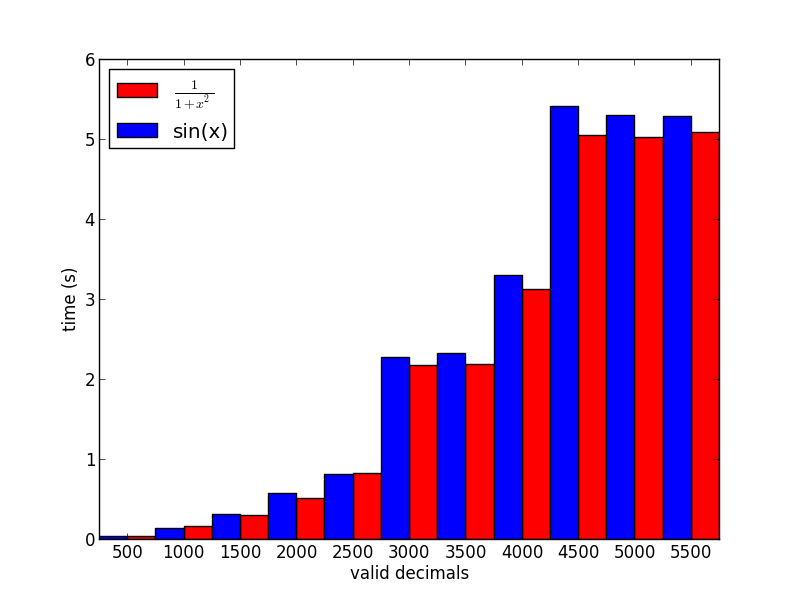
\includegraphics[width=0.5\textwidth]{img/analytic/ba_ana_dep_on_n_bar.png}
				\caption{running time evaluating \baana at fixed point $x=0.8$ depending on the desired number of valid decimals}
				\label{fig:ba_ana dep on n}
			\end{figure}
			\begin{figure}[h]
				\centering
				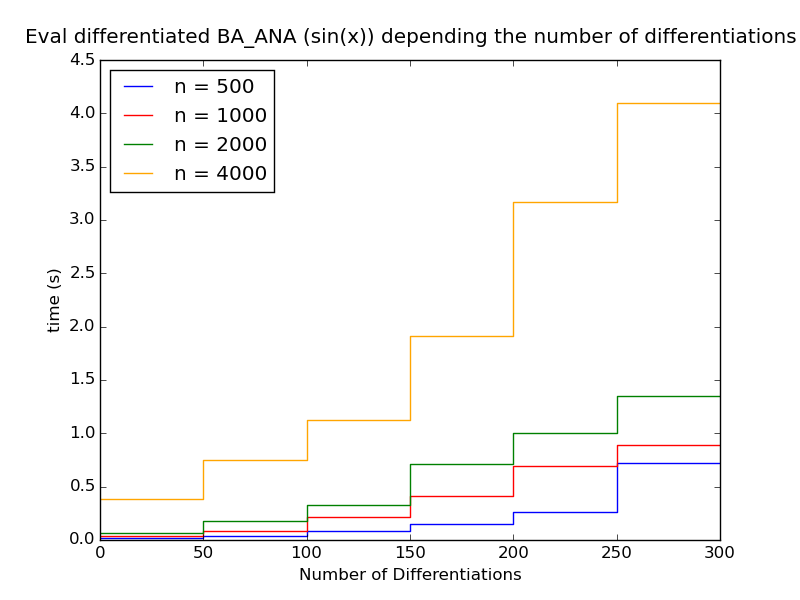
\includegraphics[width=0.5\textwidth]{img/analytic/ba_ana_dep_on_diff_sin.png}
				\caption{running time evaluating differentiated \baana with series for $\sin(x)$ at fixed point $x=0.8$ with different number
        of desired valid decimals depending on the number of differentiation}
				\label{fig:ba_ana dep on differentiation}
			\end{figure}
      All operations on \baana are expected to run in polynomial time.
      Thus, the algorithms are expected to run reasonably fast.

      This could be verified in the performed tests. 
      Figure \ref{fig:ba_ana dep on n} depicts the running time for the two real-valued functions $x \to \sin(x)$ and $x \to \frac{1}{1+x^2}$.
      Similiar results were obtained for other functions.

      Of course it's possible to compute those functions much faster, e.g. by using {\irram}'s built-in $\sin$ function.
      However to obtain the above results no special properties of those functions were used, but only the information 
      contained in the Taylor series and the two additional parameters.
      Thus, the results obtained are very general and should hold for all kind of functions (as long as the complexity to compute
      the series is similiar).

      \ref{fig:ba_ana dep on differentiation} shows how the running time depends on the number of differentiation. \temp{This picture is strange and should be replaced}

      Other operations like addition and multiplication yield similiar running times and the results are therefore omitted.

      All in all, the running times obtained for the tested examples were very close to what was expected from the theoretical analysis, and seem to
      be quite good, although due to the lack of similiar approaches to compute analytic functions, it is hard to make any comparisons.

      \subsection{\anarect}
			Since most operations on the power series on \anarect and \baana are identical‚ and are therefore expected to behave similiarily, 
			the crucial part of evaluating \baana is the evaluation using analytic continuation.
			
			In particular the following questions are interesting
			\begin{enumerate}
				\item How does the running time depend on the number of analytic continuations and on the output precision?
				\item How many coefficients of each power series are needed?
				\item How does the number of coefficients needed grow with the number of iterations and the output precision?
			\end{enumerate} 

		From the theoretical analysis, the expected behavior is that the running time for evaluating at a fixed 
		point should depend polynomially on the desired output precision $n$, bounded by $O(n^4)$.

    In the number of analytic continuations it should grow exponentially.
    
    A similiar dependency on output precision and number of analytic continuations should hold for number of coefficients that are read 
    from the original series given to the constructor of the \anarect object.


		\begin{figure}[h]
			\centering
			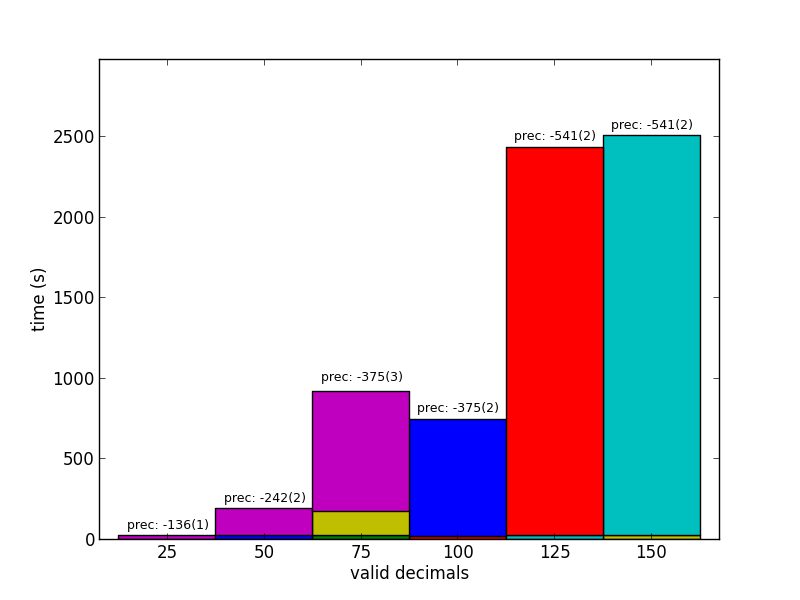
\includegraphics[width=0.5\textwidth]{img/analytic/sin_for_series_4_dep_on_n.png}
			\caption{running time of \anarect computing the sine function at the boundary of the third series, depending on the number of valid digits. The text above the bars shows the highest internal precision and the number of iterations \irram did.}
			\label{fig:sin dep on n}
		\end{figure}

		Figure \ref{fig:sin dep on n} shows, how the running time of evaluating at a fixed point $x$ depends on the desired number of valid decimals. 
		$x$ is chosen so that $3$ analytic continuations are necessary. 

		The plot also contains the information on how many iterations \irram performed and the maximum internal 
		precision (text above the bars). 
		Every bar is broken down into smaller bars, that show how much time was spent in each iteration of the \irram.

		The reason for the running time going down again between $75$ and $100$ decimals is, that
		the iterations do not always have the same size, but \irram makes estimates on a good step size.
		The internal precision in the end is $-375$ for both $n=75$ and $n=100$, but 
		for $75$ the first estimate is too small, leading to a total number of $3$ iterations instead of only $2$ iterations for $n=100$.

		However, the plot also clearly indicates that the running time is always strongly dominated by the time spent in the last iteration.

		\begin{figure}[h]
			\centering
			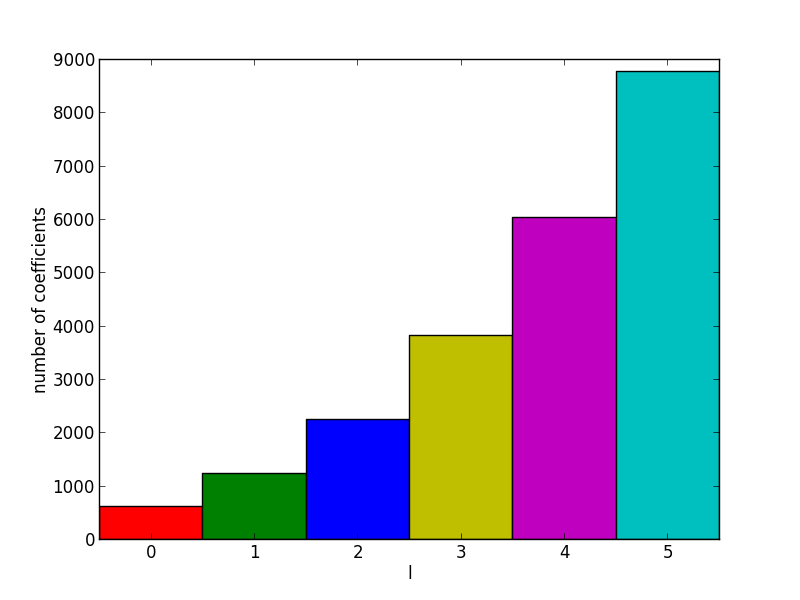
\includegraphics[width=0.5\textwidth]{img/analytic/sin_for_coeffs_prec_150_dep_on_series.png}
			\caption{Number of coefficients read from the original series when evaluating sine-function with 150 valid decimals, depending on the number of analytic continuations}
			\label{fig:sin dep on n}
		\end{figure}

		\begin{table}[h]
			 \centering
			\begin{subtable}{0.48\textwidth}
				\centering
			  	\begin{tabular}{|c|c|c|}
			  	\hline
			  	prec & $N^{(1)}$ & sec \\
			  	\hline
			  	50 & 71 & 0\\
			  	\hline
			  	136 & 271 & 0\\
			  	\hline
			  	242 & 527 & 2\\
			  	\hline
			  	375 & 842 & 6\\
			  	\hline
			  	541 & 1235 & 20\\
			  	\hline
			  	\end{tabular}
			  	\caption{evaluating at series 1}
		  	\end{subtable}
			\begin{subtable}{0.48\textwidth}
				\centering
			  	\begin{tabular}{|c|c|c|c|c|c|}
			  	\hline
			  	prec & $N^{(0)}$ & $N^{(1)}$ &$N^{(2)}$ & $N^{(3)}$ & $N^{(4)}$ \\
			  	\hline
			  	50 & 13 & 30 & 59 & 112 & 212\\
			  	\hline
			  	136 & 55 & 120 & 234 & 442 & 833\\
			  	\hline
			  	242 & 109 & 236 & 458 & 863 & 1626\\
			  	\hline
			  	375 & 175 & 378 & 733 & 1382 & 2603\\
			  	\hline
			  	541 & 258 & 556 & 1078 & 2031 & 3825\\
			  	\hline
			  	\end{tabular}
			  	\caption{evaluating at series 3}
		  	\end{subtable}
          % \begin{tabular}{|c||c|c|c|c|c|}
          % \hline
          % prec & $N^{(0)}$ & $N^{(1)}$ &$N^{(2)}$ & $N^{(3)}$ & $N^{(4)}$ \\
          % \hline\hline
          % 50 & 12 & 31 & 63 & 121 & 229\\
          % \hline
          % 136 & 55 & 136 & 276 & 531 & 1009\\
          % \hline
          % 242 & 107 & 248 & 493 & 939 & 1778\\
          % \hline
          % 375 & 175 & 393 & 773 & 1466 & 2769\\
          % \hline
          % 541 & 258 & 571 & 1118 & 2116 & 3993\\
          % \hline
          % \end{tabular}
			\caption{Number of coefficients accessed in an iRRAM iteration of precision \sprec when evaluating at on the boundary of the first and third series.}
			\label{fig:xinv coeff 0 dep on n}
		\end{table}

		Table \ref{fig:xinv coeff 0 dep on n} shows the number $N^{(l)}$ of coeffcients accesed from the original series, when evaluated at a point where $l$ analytic continuations are necessary depending on 
		the internal precision of \irram.

		\begin{figure}[h]
			\centering
			\begin{subfigure}{.45\textwidth}
				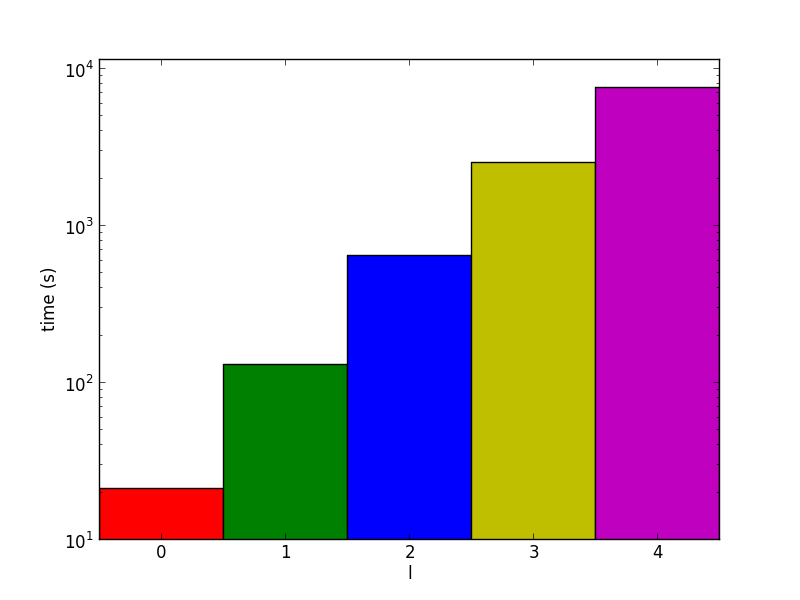
\includegraphics[width=1.0\textwidth]{img/analytic/sin_for_n_prec_150_dep_on_series_log.png}
				\caption{$\sin(x)$}
			\end{subfigure}
			\begin{subfigure}{.45\textwidth}
				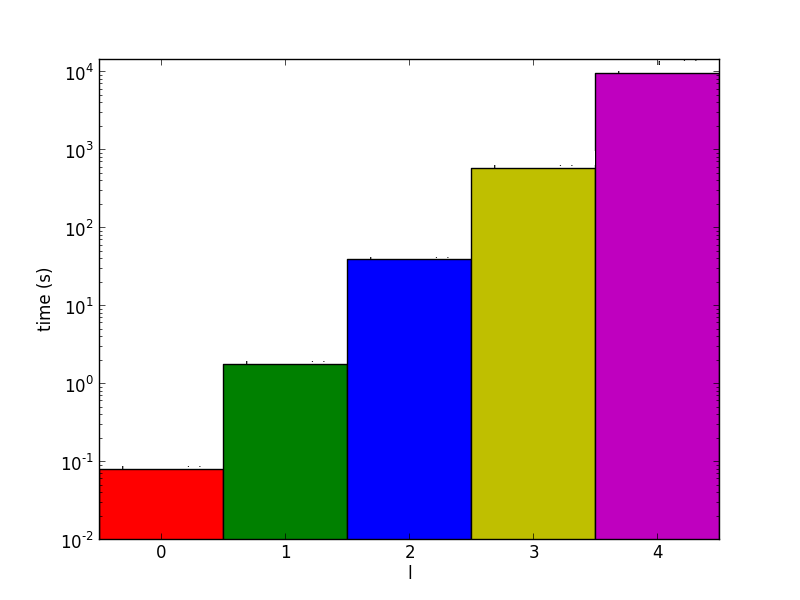
\includegraphics[width=1.0\textwidth]{img/analytic/log_for_n_prec_150_dep_on_series_log.png}
				\caption{$\log(2+x)$}
			\end{subfigure}
			\caption{log-scale plot of the running time for \anarect with 150 valid digits at the boundary of the $l$-th series.}
			\label{fig:baana dep on series}
		\end{figure}
    
    \begin{table}
      \centering
      \begin{tabular}{|c||c|c|c|c|c|c|c|}
        \hline
        precision & series 0&series 1&series 2&series 3&series 4&series 5&series 6 \\ \hline
        52 &1914&1039&576&325&185&104&55 \\ \hline 
        512 &3721&2021&1121&633&361&204&109 \\ \hline
        2300 &5978&3247&1801&1017&580&328&175 \\ \hline
        7550 &8775 & 4766 & 2644 & 1493&851&481&257 \\ \hline
      \end{tabular}
      \caption{The number of coefficients read from each series depending on {\irram}'s precision. 
    Results are for the sine function evaluated at the border of the series 6.}\label{table: coefficients dep on precision} 
    \end{table}
		How the running time and the number of coefficients depends on the number of analytic continuations can also be observed in Figure \ref{fig:baana dep on series} 
    and Table \ref{table: coefficients dep on precision}.

    It can be seen that the number of coefficients read approximately doubles in each analytic continuation and thus grows 
    a little slower than the upper bound established in the theoretical analysis.

		All in all the figures are very well in accordance with the qualitative behaviour expected from the analysis in the theory section.

  \section{Root Refinement for Real Polynomials}
  \subsection{Introduction}
  \subsection{Implementation}
  \subsection{Evaluation}
  \chapter{Conclusion}
  \section{Future Work}
  \bibliography{thesis}
\end{document}
